\chapter{METHODOLOGY}
\section{Software Model Used}
\textbf{Agile Methodology}\\
Agile methodology is the chosen approach for the development of the Quiz App, embracing the principles of flexibility, iterative development, and responsiveness to changing requirements. Unlike the traditional Waterfall model, Agile promotes continuous collaboration between cross-functional teams, allowing for incremental development and continuous user feedback. This iterative approach aligns well with the dynamic nature of educational technology projects.

\begin{figure}[h!]
    \centering
    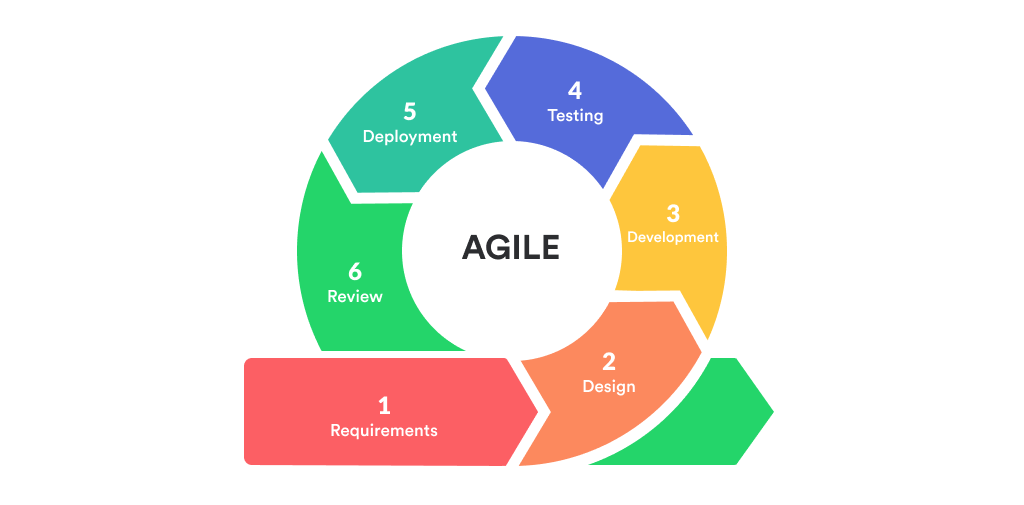
\includegraphics[scale=0.5]{project/images/Agile1.png}
    \caption{AGILE METHODOLOGY}
\end{figure}

The Agile methodology facilitates the seamless integration of different components and features, ensuring a cohesive and adaptable development process.

\section{Product User Interfaces}
The Quiz App's user interfaces are designed to provide an engaging and intuitive experience for both students and faculty members. Let's explore the various interfaces:

\subsection{Welcome Page}
\begin{center}
    \includegraphics[scale=0.4]{project/images/WELCOME.png}
\end{center}

The welcome page serves as the entry point for users, providing a visually appealing and informative introduction to the Quiz App. It sets the tone for a positive user experience.

\subsection{Login Page}
\begin{center}
    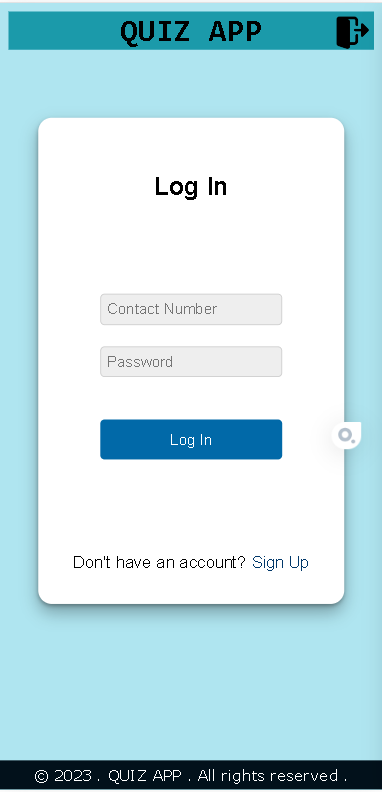
\includegraphics[scale=0.4]{project/images/LOGIN.png}
\end{center}

The login page allows users to securely access their accounts. Students and faculty members can enter their credentials to log in and access personalized features based on their roles.

\subsection{Register Page}
\begin{center}
    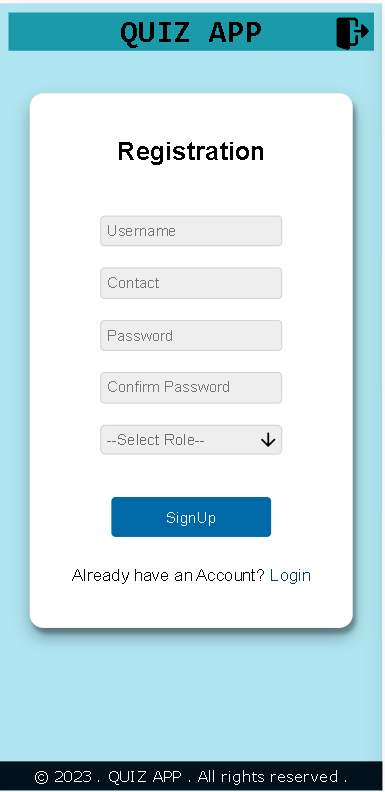
\includegraphics[scale=0.4]{project/images/REGISTER.png}
\end{center}

For new users, the register page offers a straightforward registration process. Students and faculty can create accounts by providing essential details, ensuring a seamless onboarding experience.

\subsection{Student Interface - Subject Selection}
\begin{center}
    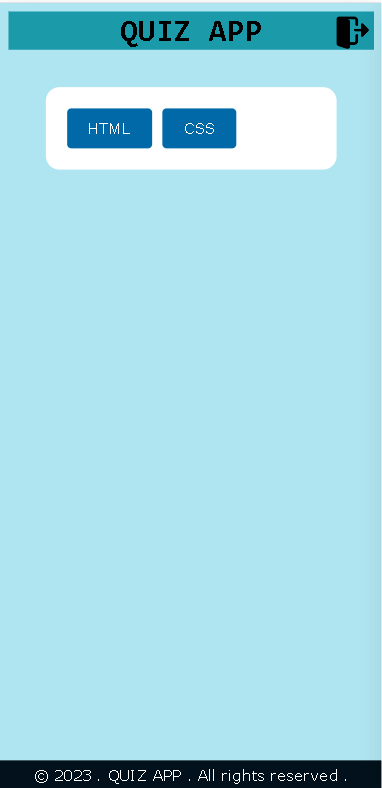
\includegraphics[scale=0.4]{project/images/QUIZ PANEL.png}
\end{center}

Students can choose quizzes based on subjects of their interest. The interface provides a user-friendly way to navigate through available subjects and select quizzes to participate in.

\subsection{Student Interface - Specific Subject Questions}
\begin{center}
    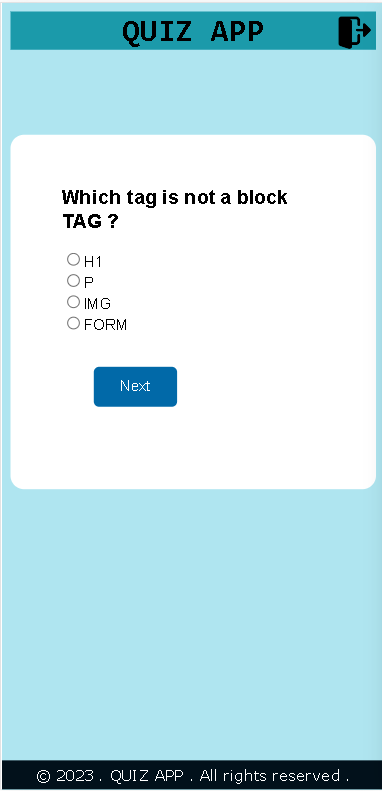
\includegraphics[scale=0.4]{project/images/QUIZ PANEL2.png}
\end{center}

For a more targeted quiz experience, students can opt for specific subject questions. This interface displays questions related to a particular subject, allowing students to focus on their areas of study.

\subsection{Faculty Interface - Add Subject}
\begin{center}
    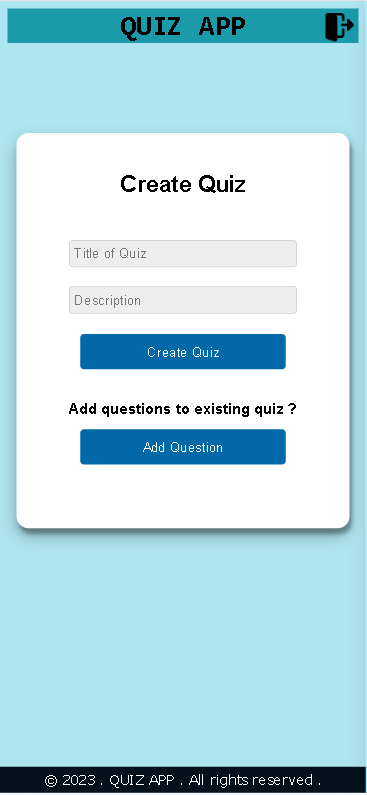
\includegraphics[scale=0.4]{project/images/ADD SUBJECT.png}
\end{center}

Faculty members have the capability to enrich the Quiz App by adding new subjects. This interface streamlines the process, ensuring efficient management of the available subjects.

\subsection{Faculty Interface - Add Question}
\begin{center}
    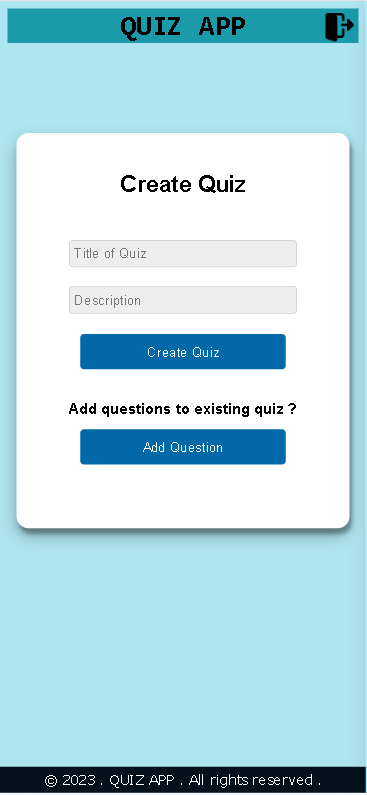
\includegraphics[scale=0.4]{project/images/ADD SUBJECT.png}
\end{center}

Facilitating continuous improvement, faculty members can contribute to the question database by adding new questions. This interface provides a structured form for adding questions, ensuring consistency in data entry.

\section{Features}

The Quiz App incorporates several features to enhance the learning and quiz-taking experience:

\begin{enumerate}
    \item \textbf{User-Friendly Interface:} The application is designed with a focus on user experience, ensuring an intuitive and navigable interface for both students and faculty members.
    \item \textbf{Quiz Selection and Submission:} Students can choose quizzes, answer questions, and submit responses for evaluation. The integration with the student API enables seamless access to quiz data.
    \item \textbf{Quiz Management:} Faculty members utilize the teacher API to manage quiz content, adding new subjects, creating questions, and organizing quizzes. This feature ensures an efficient workflow for educators.
    \item \textbf{Real-Time Data Synchronization:} The application's integration with three APIs ensures real-time updates and synchronization, providing accurate information for students and facilitating efficient content management for teachers.
\end{enumerate}

\section{Design and Implementation Constraints}

Agile principles inherently address various constraints and promote adaptability:

\begin{enumerate}
    \item \textbf{Operating System and Device Flexibility:}
    \begin{itemize}
        \item Agile development ensures that the Quiz App remains adaptable to various operating systems and devices, providing flexibility for users with different preferences.
    \end{itemize}
    
    \item \textbf{Continuous Integration and Testing:}
    \begin{itemize}
        \item Agile's continuous integration and testing practices help identify and address potential constraints early in the development process, ensuring a robust and reliable application.
    \end{itemize}
\end{enumerate}

The Agile methodology aligns with the Quiz App's goals, fostering collaboration, adaptability, and delivering a product that meets the evolving needs of students and faculty.
